\documentclass[10pt]{article}
\usepackage{amsmath,amssymb}
\setlength{\oddsidemargin}{0in}
\setlength{\evensidemargin}{0in}
\setlength{\textheight}{9in}
\setlength{\textwidth}{6.5in}
\setlength{\topmargin}{-0.5in}
\usepackage{enumitem}
\usepackage[table]{xcolor}
\usepackage{graphicx}
\usepackage{tikz,pgfplots}
\usetikzlibrary{positioning}
\usetikzlibrary{calc}
\usetikzlibrary{patterns}
\usetikzlibrary{shapes.geometric}
\pgfplotsset{compat=1.18}
\usepackage{hyphenat}


\title{\bf Math 131B: Homework 1}
\date{4/14/2023}
\author{\bf Owen Jones}

\begin{document}
\maketitle

\begin{enumerate}[label=\bfseries Problem \arabic*:]
    \item \textbf{Exercise 1.1.5:}\\
    We will complete a proof by induction on $n$ to show $(\displaystyle{\sum_{i=1}^{n}}a_ib_i)^2
    +\frac{1}{2}\displaystyle{\sum_{i=1}^{n}}\displaystyle{\sum_{j=1}^{n}} (a_ib_j-a_jb_i)^2
    =(\displaystyle{\sum_{i=1}^{n}}a_i)^2(\displaystyle{\sum_{i=1}^{n}}b_i)^2$ is true for all $n$.
    We will denote the statement $P(n):(\displaystyle{\sum_{i=1}^{n}}a_ib_i)^2
    +\frac{1}{2}\displaystyle{\sum_{i=1}^{n}}\displaystyle{\sum_{j=1}^{n}} (a_ib_j-a_jb_i)^2
    =(\displaystyle{\sum_{i=1}^{n}}a_i)^2(\displaystyle{\sum_{i=1}^{n}}b_i)^2$.\\
   
    Base case: The LHS of $P(1): (\displaystyle{\sum_{i=1}^{1}}a_ib_i)^2+\frac{1}{2}\displaystyle{\sum_{i=1}^{1}}\displaystyle{\sum_{j=1}^{1}}(a_ib_j-a_jb_i)^2$
    and the RHS of $P(1): (\displaystyle{\sum_{i=1}^{1}}a_{i}^2)(\displaystyle{\sum_{i=1}^{1}}b_{i}^2)$ are both equal to $a_{1}^{2}b_{1}^{2}$.
    Since the left-hand-side and the right-hand-side are equal, the statement $P(1)$ holds.\\
    Induction hypothesis: Assume for some arbitrary $n\ge1$ the statement $P(n)$ holds.\\
    Induction step: It remains to show the statement $P(n+1)$ holds by manipulating the LHS of $P(n+1)$ to look like the RHS.\\
    First, foil $(\displaystyle{\sum_{i=1}^{n+1}}a_ib_i)^2=(a_1b_1+a_2b_2+...+a_{n+1}b_{n+1})(a_1b_1+a_2b_2+...+a_{n+1}b_{n+1})=\displaystyle{\sum_{i=1}^{n+1}}\displaystyle{\sum_{j=1}^{n+1}}a_ib_ia_jb_j$\\
    Second, foil $\frac{1}{2}\displaystyle{\sum_{i=1}^{n+1}}\displaystyle{\sum_{j=1}^{n+1}}(a_ib_j-a_jb_i)^2\\
    =\frac{1}{2}\displaystyle{\sum_{i=1}^{n+1}}\displaystyle{\sum_{j=1}^{n+1}}a_{i}^{2}b_{j}^{2}-2a_ib_ia_jb_j+a_{j}^{2}b_{i}^{2}\\
    =\frac{1}{2}\displaystyle{\sum_{i=1}^{n+1}}\displaystyle{\sum_{j=1}^{n+1}}a_{i}^{2}b_{j}^{2}-\displaystyle{\sum_{i=1}^{n+1}}\displaystyle{\sum_{j=1}^{n+1}}a_ib_ia_jb_j+\frac{1}{2}\displaystyle{\sum_{i=1}^{n+1}}\displaystyle{\sum_{j=1}^{n+1}}a_{j}^{2}b_{i}^{2}$\\
    We can swap the index variables $j$ and $i$, so $\frac{1}{2}\displaystyle{\sum_{i=1}^{n+1}}\displaystyle{\sum_{j=1}^{n+1}}a_{j}^{2}b_{i}^{2}=\frac{1}{2}\displaystyle{\sum_{i=1}^{n+1}}\displaystyle{\sum_{j=1}^{n+1}}a_{i}^{2}b_{j}^{2}$\\
    $\Rightarrow \frac{1}{2}\displaystyle{\sum_{i=1}^{n+1}}\displaystyle{\sum_{j=1}^{n+1}}(a_ib_j-a_jb_i)^2= \displaystyle{\sum_{i=1}^{n+1}}\displaystyle{\sum_{j=1}^{n+1}}a_{i}^{2}b_{j}^{2}-\displaystyle{\sum_{i=1}^{n+1}}\displaystyle{\sum_{j=1}^{n+1}}a_ib_ia_jb_j$\\
    Thus, the LHS of $P(n+1)$ is equivalent to $\displaystyle{\sum_{i=1}^{n+1}}\displaystyle{\sum_{j=1}^{n+1}}a_{i}^{2}b_{j}^{2}$\\
    Factoring the above, we obtain $\displaystyle{\sum_{i=1}^{n+1}}\displaystyle{\sum_{j=1}^{n+1}}a_{i}^{2}b_{j}^{2}=(a_{1}^{2}+a_{2}^{2}+...+a_{n+1}^{2})(b_{1}^{2}+b_{2}^{2}+...+b_{n+1}^{2})=(\displaystyle{\sum_{i=1}^{n+1}}a_{i}^{2})(\displaystyle{\sum_{i=1}^{n+1}}b_{i}^{2})$ \\which is exactly the RHS of $P(n+1)$. Thus, $P(n+1)$ holds.\\
    Hence, by induction, $P(n)$ holds for all $n$.\\
    QED
    \\
    \\
    \\
    Because the square of a number is always non-negative\\
    $(\displaystyle{\sum_{i=1}^{n}}a_ib_i)^2\le (\displaystyle{\sum_{i=1}^{n}}a_ib_i)^2+\frac{1}{2}\displaystyle{\sum_{i=1}^{n}}\displaystyle{\sum_{j=1}^{n}}(a_ib_j-a_jb_i)^2\le (\displaystyle{\sum_{i=1}^{n}}a_{i}^2)(\displaystyle{\sum_{i=1}^{n}}b_{i}^2)$\\
    Taking the square root of both sides\\
    $|\displaystyle{\sum_{i=1}^{n}}a_ib_i|\le \sqrt{\displaystyle{\sum_{i=1}^{n}}a_{i}^2}\sqrt{\displaystyle{\sum_{i=1}^{n}}b_{i}^2}$\\
    Thus, we obtain the Cauchy-Schwarz innequality.\\
    QED
    \\
    \\
    \\
    Foiling $(a_i+b_i)^2$, we obtain $\sqrt{\displaystyle{\sum_{i=1}^{n}}(a_i+b_i)^2}=\sqrt{\displaystyle{\sum_{i=1}^{n}}a_i^2+2\displaystyle{\sum_{i=1}^{n}}a_ib_i+\displaystyle{\sum_{i=1}^{n}}b_i^2}$\\
    Using the Cauchy-Schwarz innequality, $\sqrt{\displaystyle{\sum_{i=1}^{n}}a_i^2+2\displaystyle{\sum_{i=1}^{n}}a_ib_i+\displaystyle{\sum_{i=1}^{n}}b_i^2}\le \sqrt{\displaystyle{\sum_{i=1}^{n}}a_i^2+2\sqrt{\displaystyle{\sum_{i=1}^{n}}a_{i}^2}\sqrt{\displaystyle{\sum_{i=1}^{n}}b_{i}^2}+\displaystyle{\sum_{i=1}^{n}}b_i^2}$\\
    Factoring $\sqrt{\displaystyle{\sum_{i=1}^{n}}a_i^2+2\sqrt{\displaystyle{\sum_{i=1}^{n}}a_{i}^2}\sqrt{\displaystyle{\sum_{i=1}^{n}}b_{i}^2}+\displaystyle{\sum_{i=1}^{n}}b_i^2}$ we obtain $\sqrt{(\sqrt{\displaystyle{\sum_{i=1}^{n}}a_i}+\sqrt{\displaystyle{\sum_{i=1}^{n}}b_i})^2}$\\
    Cancelling the square with the square root, we obtain $|\sqrt{\displaystyle{\sum_{i=1}^{n}}a_{i}^{2}}+\sqrt{\displaystyle{\sum_{i=1}^{n}}b_{i}^{2}}|=\sqrt{\displaystyle{\sum_{i=1}^{n}}a_{i}^{2}}+\sqrt{\displaystyle{\sum_{i=1}^{n}}b_{i}^{2}}$\\
    $\Rightarrow\sqrt{\displaystyle{\sum_{i=1}^{n}}(a_i+b_i)^2}\le\sqrt{\displaystyle{\sum_{i=1}^{n}}a_{i}^2}+\sqrt{\displaystyle{\sum_{i=1}^{n}} b_{i}^{2}}$\\
    Thus, we obtain the triangle innequality.\\
    QED
    \newpage
    \item \textbf{Exercise 1.1.6:}
    \begin{itemize}
        \item [a)] For $x\in \mathbf{R}^n$ $d(x,x)=\sqrt{\displaystyle{\sum_{i=1}^{n}}(x_i-x_i)^2}=\sqrt{\displaystyle{\sum_{i=1}^{n}}0}=0$
        \item [b)] For $x,y\in \mathbf{R}^n$ $d(x,y)=\sqrt{\displaystyle{\sum_{i=1}^{n}}(x_i-y_i)^2}\ge0$ because the square of a number is always non-negative.
        \item [c)] For $x,y\in \mathbf{R}^n$ $d(x,y)=\sqrt{\displaystyle{\sum_{i=1}^{n}}(x_i-y_i)^2}=\sqrt{\displaystyle{\sum_{i=1}^{n}}(y_i-x_i)^2}=d(y,x)$
        \item [d)] For $x,y,z\in \mathbf{R}^n$ $d(x,y)=\sqrt{\displaystyle{\sum_{i=1}^{n}}(x_i-y_i)^2}=\sqrt{\displaystyle{\sum_{i=1}^{n}}((x_i-z_i)+(z_i-y_i))^2}\le\sqrt{\displaystyle{\sum_{i=1}^{n}}(x_i-z_i)^2}+\sqrt{\displaystyle{\sum_{i=1}^{n}}(y_i-z_i)^2}=d(x,z)+d(y,z)$ by the Cauchy-Schwarz innequality.
    \end{itemize}
    Hence, $d(\mathbf{R}^n,d_{l1})$ is a metric space.\\
    QED
    
    \item \textbf{Exercise 1.1.16}\\
    $(\Rightarrow)$By the triangle innequality, $\displaystyle{\lim_{n\rightarrow\infty}} d(x_n,y_n)\le \displaystyle{\lim_{n\rightarrow\infty}} (d(x_n,x)+d(y_n,x))\le \displaystyle{\lim_{n\rightarrow\infty}} (d(x_n,x)+d(y_n,y)+d(y,x))$\\
    Because $x_n$ converges to $x$ and $y_n$ converges to $y$, $\displaystyle{\lim_{n\rightarrow\infty}}(d(x_n,x)d(y_n,y))=0$\\
    Thus, $\displaystyle{\lim_{n\rightarrow\infty}} d(x_n,y_n)\le d(x,y)$\\
    $(\Leftarrow)$ Similar to the forward direction, we can use the triangle innequality to show $d(x,y)\le\displaystyle{\lim_{n\rightarrow\infty}}d(x,x_n)+d(y,x_n)\le\displaystyle{\lim_{n\rightarrow\infty}}(d(x,x_n)+d(y,y_n)+d(x_n,y_n))$\\
    Because $x_n$ converges to $x$ and $y_n$ converges to $y$, $\displaystyle{\lim_{n\rightarrow\infty}}(d(x_n,x)d(y_n,y))=0$\\
    Thus $d(x,y)\le \displaystyle{\lim_{n\rightarrow\infty}} d(x_n,y_n)$\\
    Because $d(x,y)\le \displaystyle{\lim_{n\rightarrow\infty}} d(x_n,y_n)$ and $d(x,y)\ge \displaystyle{\lim_{n\rightarrow\infty}} d(x_n,y_n)$, this implies $d(x,y)=\displaystyle{\lim_{n\rightarrow\infty}} d(x_n,y_n)$
    QED
    
    \item \textbf{Exercise 1.2.2}\\
    We WTS $a\Rightarrow b$ then $b\Rightarrow c$ then $c\Rightarrow a$
    \begin{itemize}
        \item [1)]$a\Rightarrow b$\\
        If $x_0$ is an adherent point, $\forall r>0,B(x_0,r)\cap E\neq \emptyset$\\
        The definition of an exterior point is the logical negation of an adherent point. This implies $x_0$ is not an exterior point of $E$.\\
        Since $x_0$ is not an exterior point of $E$, it must either be an interior or boundary point.
        \item [2)]$b\Rightarrow c$\\
        If $x_0$ is an interior point of $E$ $\exists r_1>0$ s.t $B(x_0,r)\subset E$\\
        If $x_0$ is a boundary point of  $E$ $\forall r>0$ $\exists x \in B(x_0,r)$ s.t $x \in E$.\\
        In either case, we can construct a sequence $x_n$ s.t $\forall n \in \mathbb{N}$ choose $x_n\in E$ s.t $d(x_n,x)<\frac{r_1}{n}\Rightarrow \displaystyle{\lim_{n\rightarrow\infty}}d(x_n,x)=0$\\
        Thus, there exists a sequence ${(x_n)}_{n=1}^{\infty}$ in $E$ that converges to $x_0$.
        \item [3)] $c\Rightarrow a$\\
        We will prove this by contradiction.\\
        Assume to the contrary there exists a sequence ${(x_n)}_{n=1}^{\infty}$ in $E$ that converges to $x_0$ and $x_0$ is an exterior point i.e $\exists r>0$ s.t $B(x_0,r)\cap E=\emptyset$.\\
        It follows if $d(x_0,x_n)<r$ $\exists n \in \mathbb{N}$ s.t $x_n \notin E$.
        This is a contradiction because ${(x_n)}_{n=1}^{\infty}$ is a sequence in $E$.\\
        Thus, $x_0$ must be an adherent point.
    \end{itemize}
    By transitivity $a \Leftrightarrow b \Leftrightarrow c$ (i.e if $a \Rightarrow b$ and $b \Rightarrow c$ then $a \Rightarrow c$). Thus, a,b, and c are equivalent.\\
    QED
    \item \textbf{Exercise 1.2.4}
    \begin{itemize}
    \item [a)] We will prove this by contradiction\\
    Assume to the contrary $\exists x \in \overline{B}$ s.t $x \notin C$ $\Rightarrow d(x,x_0)>r$.\\
    By density, $\exists a$ s.t $d(x,x_0)-r>a>0$.\\
    By Prop 1.2.10, since $x$ is an adherent point of B, there exists a sequence ${(x_n)}_{n=1}^{\infty}$ in $B$ s.t $\displaystyle{\lim_{n\rightarrow \infty}}x_n=x$.\\
    This is a contradiction because by the triangle innequality, $\displaystyle{\lim_{n\rightarrow \infty}}d(x,x_n)\ge \displaystyle{\lim_{n\rightarrow \infty}}d(x,x_0)-d(x_n,x_0)>r+a-r=a>0\Rightarrow\displaystyle{\lim_{n\rightarrow \infty}}d(x_n,x)\neq 0$.\\
    Hence, $d(x,x_0)\le r\Rightarrow x\in C$.
    \item [b)] Let $(\mathbb{R},d_{disc})$ be the metric space with $r=1, x_0=0,$\\
    $\overline{B}={0},C=\mathbb{R}\Rightarrow\overline{B}\subset C$ and $\overline{B}\neq C$
    \end{itemize}
    \item \textbf{Additional Problems}
    \begin{itemize}
        \item [a)]
        \begin{tikzpicture}
            \draw[dashed] (0,0) circle (1);
            \fill[pattern=crosshatch dots] (0,0) circle (1);
            \draw[fill] (0.705,0.705) circle (0.04);
            \node at (1,1.3) {($\frac{\sqrt{2}}{2}$,$\frac{\sqrt{2}}{2}$)};
            \draw[help lines, color=gray!30, dashed] (-2,-2) grid (2,2);
            \draw[->,ultra thick] (-2,0)--(2,0) node[right]{$x$};
            \draw[->,ultra thick] (0,-2)--(0,2) node[above]{$y$};
        \end{tikzpicture} 
        \item [b)]
        \begin{tikzpicture}
            \draw[dashed] (0,-1) -- (-1,0) -- (0,1) --(1,0)--(0,-1);
            \fill[pattern=crosshatch dots] (0,-1) -- (-1,0) -- (0,1) --(1,0)--(0,-1);
            \draw[fill] (1,0) circle (0.04);
            \node at (1.3,0.3) {(1,0)};
            \draw[fill] (0,1) circle (0.04);
            \node at (-0.5,1.3) {(0,1)};
            \draw[fill] (-1,0) circle (0.04);
            \node at (-1.3,-0.3) {(-1,0)};
            \draw[fill] (0,-1) circle (0.04);
            \node at (0.5,-1.3) {(0,-1)};
            \draw[help lines, color=gray!30, dashed] (-2,-2) grid (2,2);
            \draw[->,ultra thick] (-2,0)--(2,0) node[right]{$x$};
            \draw[->,ultra thick] (0,-2)--(0,2) node[above]{$y$};
        \end{tikzpicture} 
        \item [c)]
        \begin{tikzpicture}
            \draw[dashed] (1,-1) -- (-1,-1) -- (-1,1) --(1,1)--(1,-1);
            \fill[pattern=crosshatch dots] (1,-1) -- (-1,-1) -- (-1,1) --(1,1)--(1,-1);
            \draw[fill] (1,1) circle (0.04);
            \node at (1.3,1.3) {(1,1)};
            \draw[fill] (1,-1) circle (0.04);
            \node at (1.3,-1.3) {(1,-1)};
            \draw[fill] (-1,-1) circle (0.04);
            \node at (-1.3,-1.3) {(-1,-1)};
            \draw[fill] (-1,1) circle (0.04);
            \node at (-1.3,1.3) {(-1,1)};
            \draw[help lines, color=gray!30, dashed] (-2,-2) grid (2,2);
            \draw[->,ultra thick] (-2,0)--(2,0) node[right]{$x$};
            \draw[->,ultra thick] (0,-2)--(0,2) node[above]{$y$};
        \end{tikzpicture} 
        \item [d)]
        \begin{tikzpicture}
            \draw[fill] (0,0) circle (0.1);
            \node at (0.4,0.3) {(0,0)};
            \draw[help lines, color=gray!30, dashed] (-2,-2) grid (2,2);
            \draw[->,ultra thick] (-2,0)--(2,0) node[right]{$x$};
            \draw[->,ultra thick] (0,-2)--(0,2) node[above]{$y$};
        \end{tikzpicture}
    \end{itemize}
    \item \textbf{Additional Problems}\\
    Let $x_0$ and $r$ be arbitrary.\\
    $\forall x \in V(x_0,r)$ choose $\epsilon(x)<d(x,x_0)-r$.\\
    WTS, for any x, $B(x,\epsilon(x))\subset V(x_0,r)$.\\
    It suffices to show, for some arbitrary $b \in B(x,\epsilon(x))$, $d(b,x_0)>r \Rightarrow b \in V(x_0,r)$.\\
    By the triangle innequality, $d(x_0,b)\ge d(x_0,x)-d(x,b)$.\\
    $x \in V(x_0,r)\Rightarrow d(x_0,x)>r$ and $b \in B(x,\epsilon(x))\Rightarrow d(x,b)<\epsilon(x)<d(x,x_0)-r$.\\
    It follows $d(x_0,x)-d(x,b)>r\Rightarrow d(x_0,b)>r\Rightarrow b \in V(x_0,r)$.\\
    Thus, $B(x,\epsilon(x))\subset V(x_0,r)$ for any $x \in V(x_0,r)\Rightarrow$ $x$ is an interior point of $V(x_0,r)$, $\forall x \in V(x_0,r)$.\\
    Hence, $V(x_0,r)$ is an open set.
\end{enumerate}
\end{document}